\label{ch:results}

The results of this work will be presented in the visual analysis of the result of the visualizations and in numerical evaluations.
%
It is necessary to compare the different projections methods and the different methods for vertical positioning,
%
and the used datasets are the generated ones from previous sections and the traffic data.

\section{Projections comparisons}

In Figures~\ref{fig:generated-datasets-dimensionality-reduction}~and~\ref{fig:generated-datasets-spatial-indexing} are shown the results of the projection method applied to the generated datasets (vertical, diagonal, 'L', 'X'), all events are shown with the same size and with the same vertical position, the object is just to verify the ordering.
%
The characteristics that are going to be looked are: if objects of the same sequence (color) are projects together, if the objects of the same sequence (color) are projected with sequential coherence (gradual change in color) and if the different sequences are projected in a coherent manner.
For this comparison, we are using the greedy vertical positioning method.

Starting on the analysis of Fig.~\ref{fig:generated-datasets-dimensionality-reduction}, we will look at each dataset and compare the visual representation of the dimensionality reduction methods.
%

\begin{figure}
    \centering
    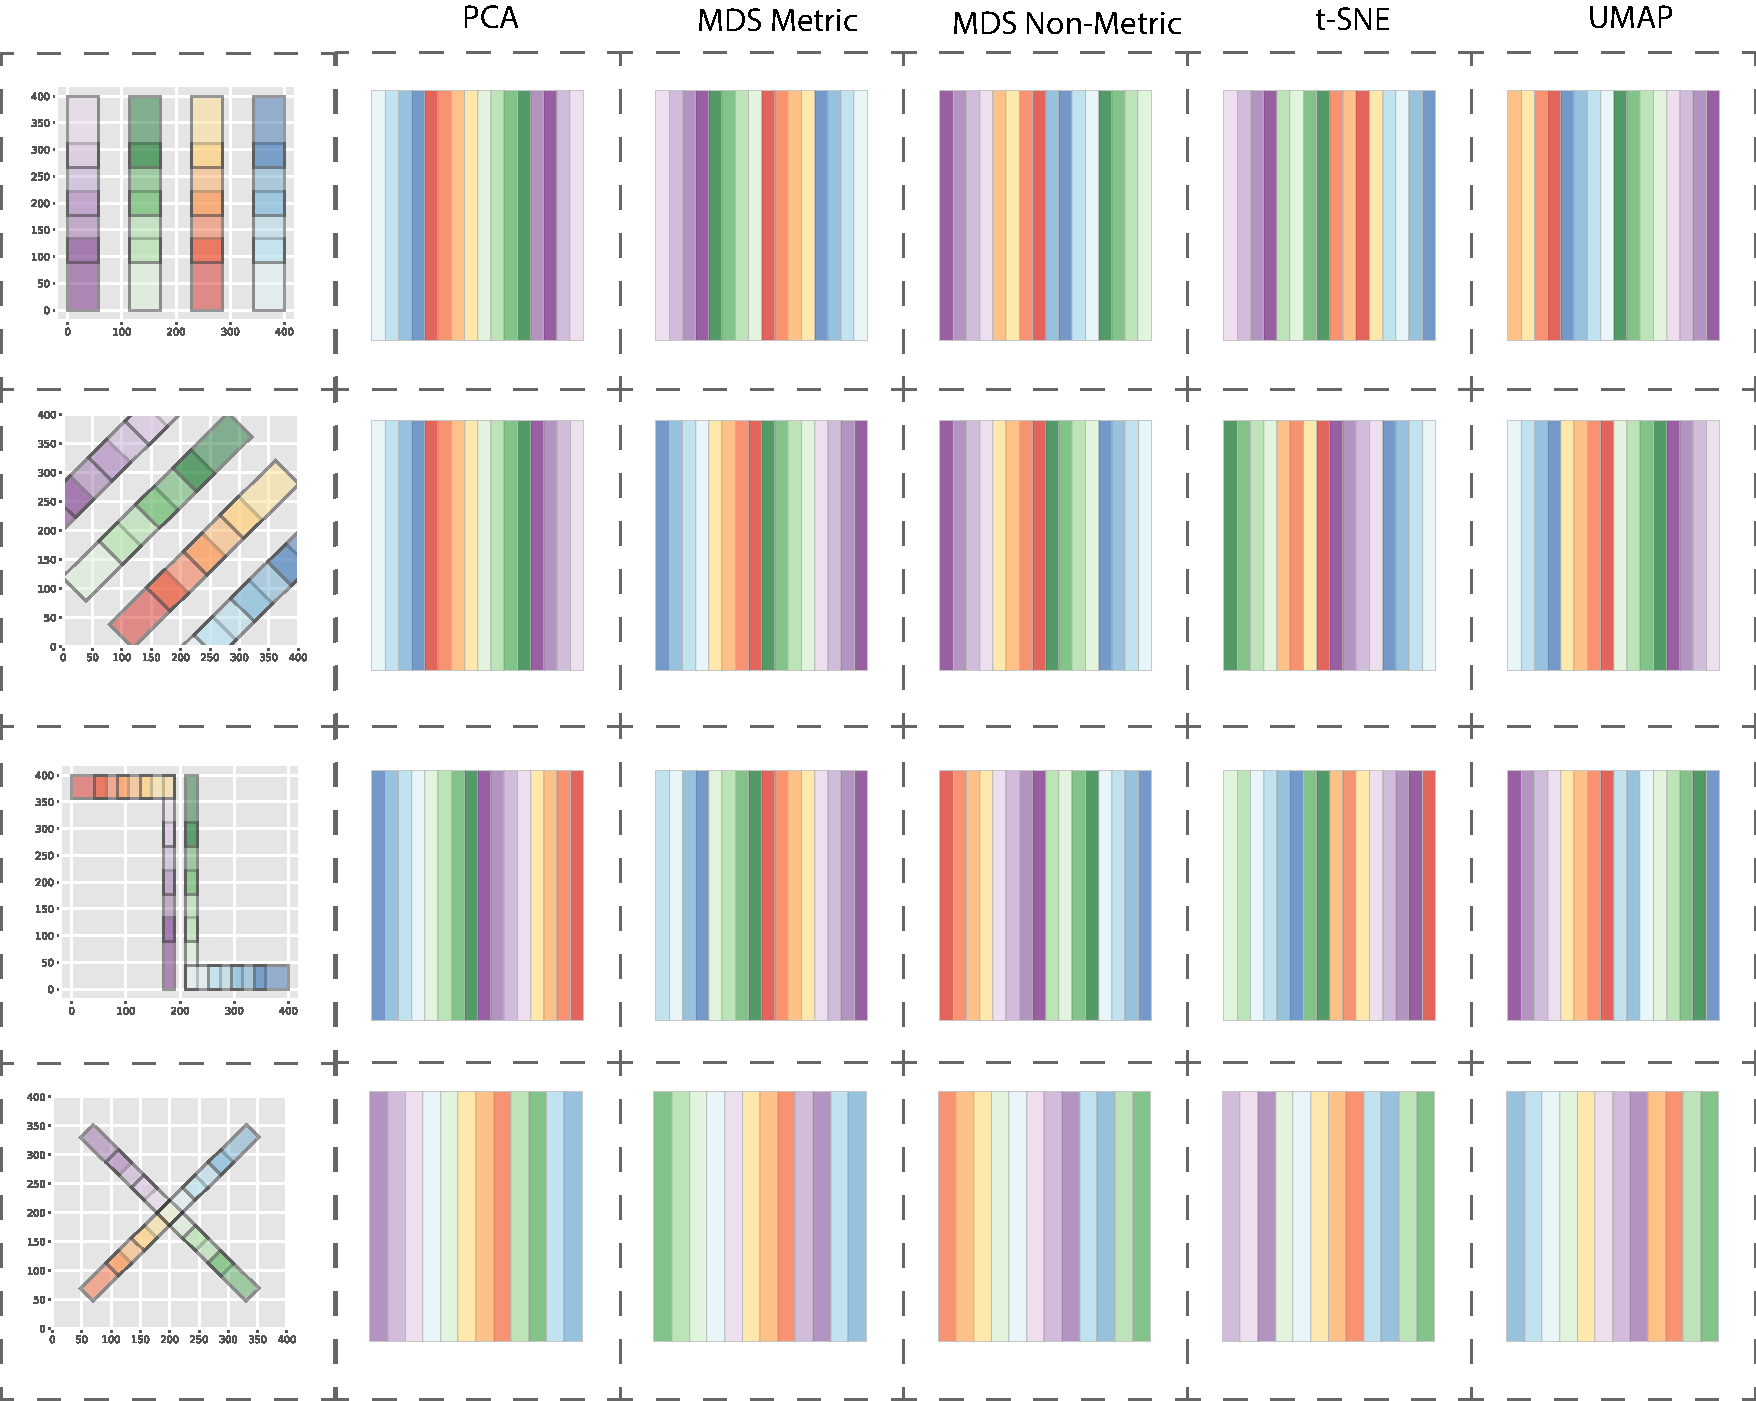
\includegraphics[width = \textwidth]{src/imgs/generated-datasets-dimensionality-reduction.pdf}
    \caption{Source: elaborated by author. Ordering of events using the generated datasets and different dimensionality reduction methods. The events are placed horizontally based on the projection ordering.}
    \label{fig:generated-datasets-dimensionality-reduction}
\end{figure}


\begin{itemize}
    \item \textit{Vertical} dataset: all projection methods kept the events from the same sequence (column) together, with mostly gradual changes in color. However, PCA, MDS-Metric, and t-SNE were able to keep the horizontal order of columns: purple, green, orange, blue (or the inverse). MDS-Metric contained the most gradual smooth inside each sequence.
    \item \textit{Diagonal} dataset: both PCA, MDS and UMAP had a good quality of representation, but the t-SNE mixed the order of diagonals. The result of UMAP was better than the previous.
    \item \textit{"L"} dataset: the PCA represented the order of columns based on the horizontal order. MDS-Metric and Non-Metric created discontinuities inside the sequences. UMAP and t-SNE mixed sequences.
    \item \textit{"X"} dataset: is the hardest to represent in 1-dimension due to the mix of the colors in the center.
    The most common representation was to show objects of the center and after the darker colors outer events, PCA, MDS-Metric and MDS Non-Metric showed this results.
    With t-SNE there was a mix between dark and lighter colors, and UMAP mixed some blue events and a dark red event.
\end{itemize}

Now analyzing Figure~\ref{fig:generated-datasets-spatial-indexing}, we analyze the results with spatial indexing methods and compare the different orders of the space-filling curve. Looking at each dataset:

\begin{figure}
    \centering
    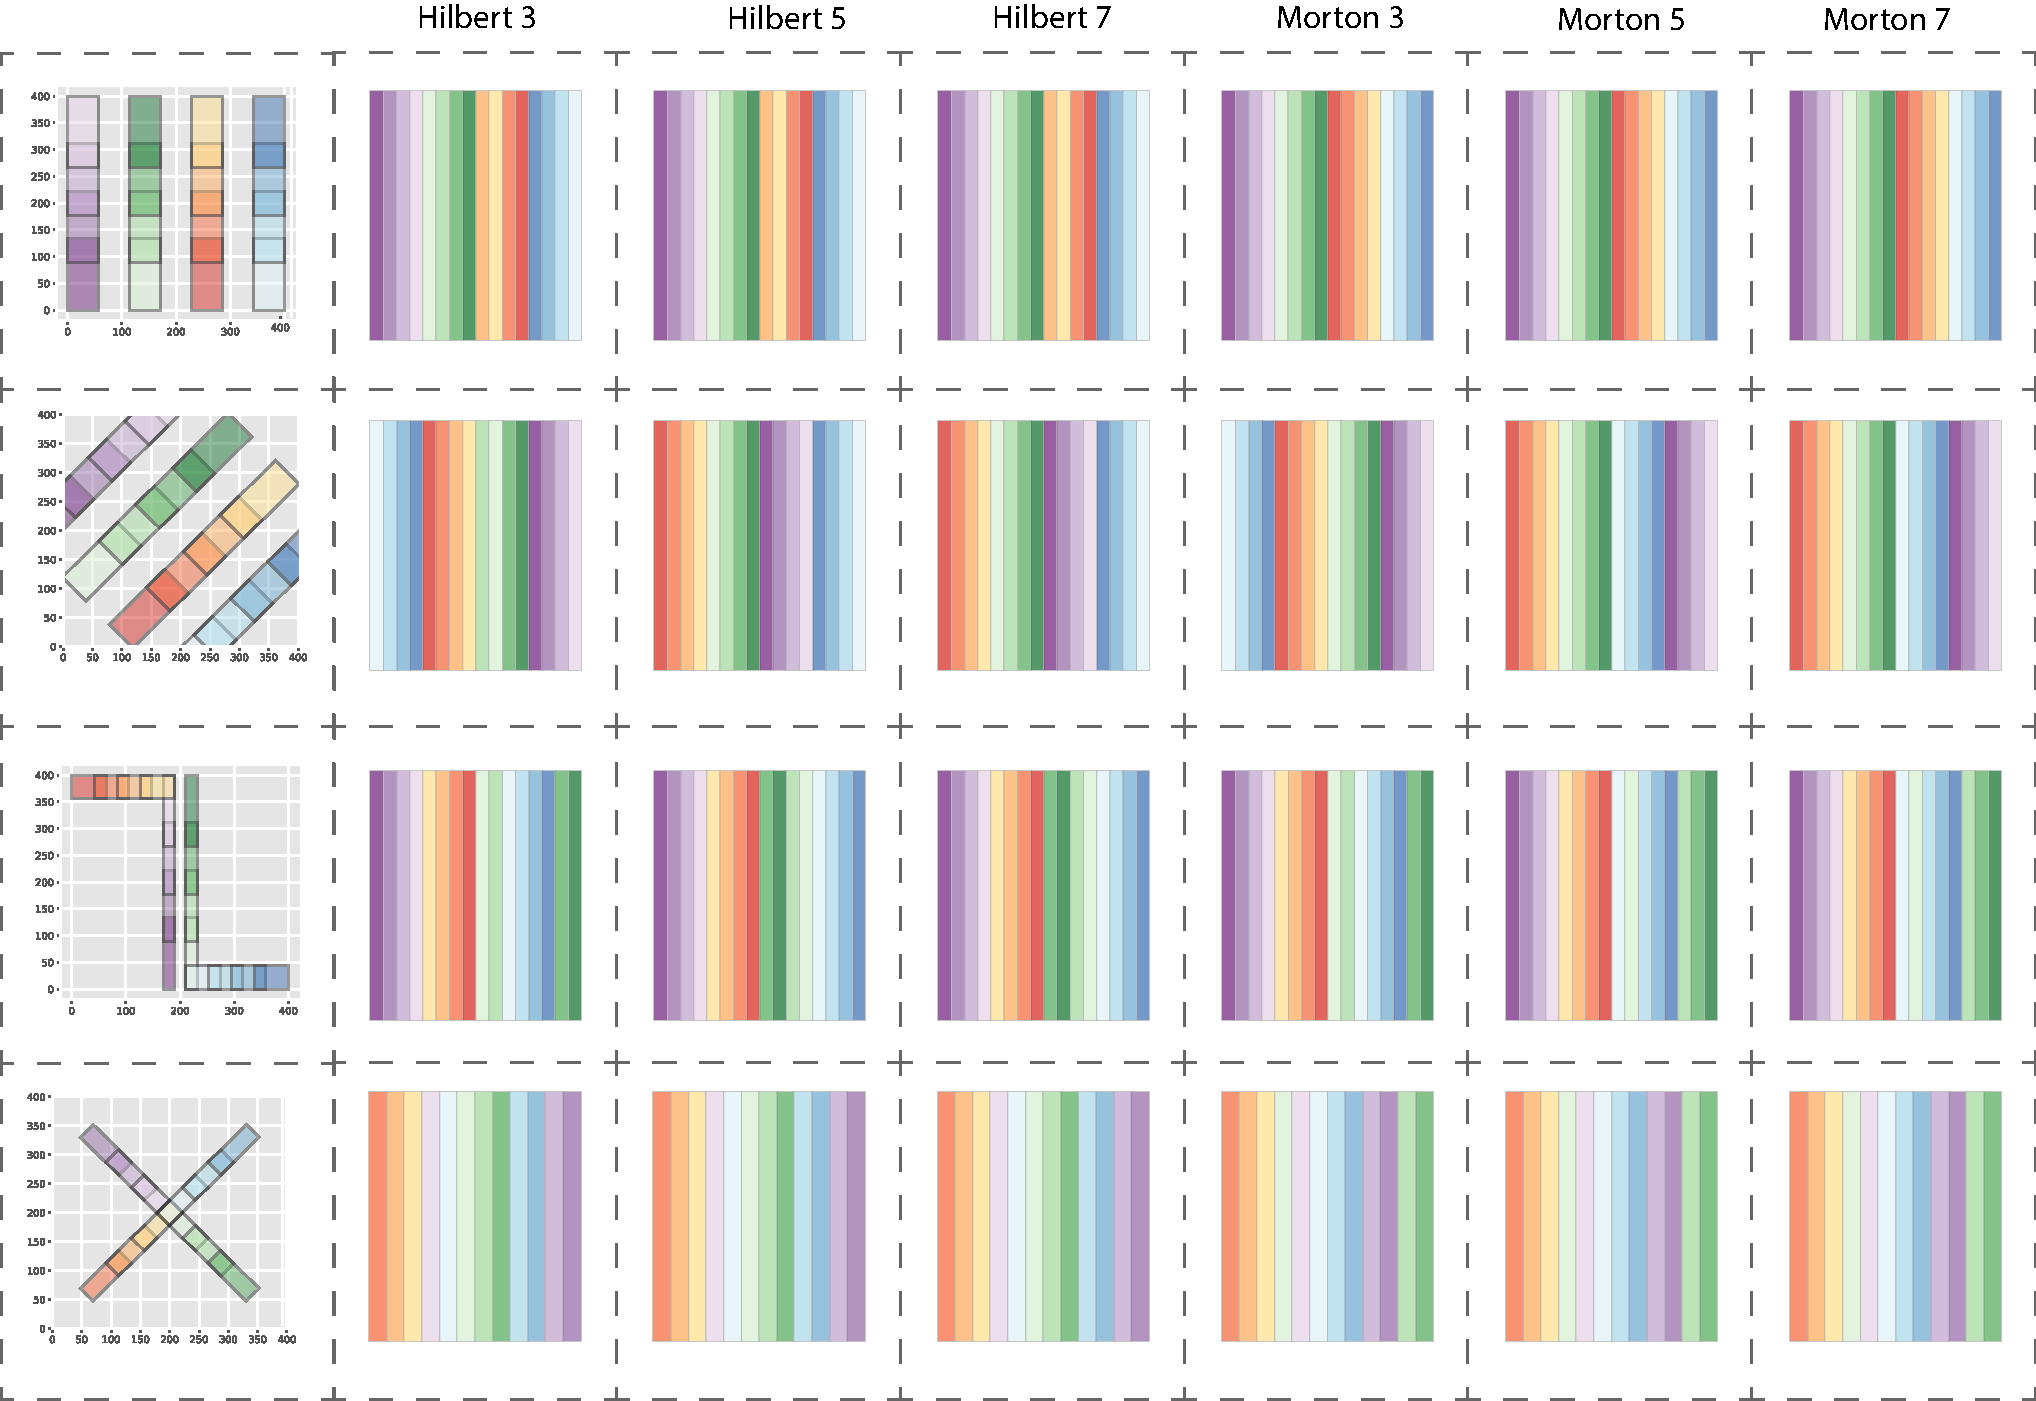
\includegraphics[width = \textwidth]{src/imgs/generated-datasets-spatial-indexing.pdf}
    \caption{Source: elaborated by author. Ordering of events using the generated datasets and different spatial indexing methods. The events are placed horizontally based on the projection ordering.}
    \label{fig:generated-datasets-spatial-indexing}
\end{figure}

\begin{itemize}
    \item \textit{Vertical} dataset: All methods were able to preserve the different columns of events, and all results were the same independently of the order of the curve. Hilbert presented discontinuities on the red sequence, while Morton ordered it gradually.
    \item \textit{Diagonal} dataset: It is possible to view changes from the curve of order 3 to order 5, although the events are making jumps from the color blue to the color purple in the curves or order 5 and 7, opposite sides of the space.
    \item \textit{"L"} dataset:  The ordering is again pretty similar in all curves, with changes from order 3 to order 5 on the Hilbert curve. In all cases, the sequences were not placed following a direction.
    \item \textit{"X"} dataset: the hardest dataset for dimensionality reductions method, showed similar results with spatial-indexing. All curves started with red events, exhibited events of light  color. The dark colors were placed gradually.
\end{itemize}





We also analyze the numeric error values for the different projection methods.
%
The numeric results confirm our previous commentaries, it is possible to identify the best results considering the stress measure on all datasets is with the use of the PCA.
%
The space-filling curves were the second best, with really similar values to PCA, with the exception of the \textit{Rotated} dataset, where they were the worst projection method.
%

Regarding the neighborhood error, the results were similar in all projections with all datasets. One special case is the \textit{L} dataset where the curves Hilbert of orders 5 and 7 had a smaller value than the other space-filling curves.
%
Looking now at the processing time, the use of the UMAP projection method is the only one that passed on second, presenting no advantage in comparison with the other methods.

\begin{table}[tb]
\centering
\resizebox{0.4\linewidth}{!}{%
\begin{tabular}{
    c |
	S[table-number-alignment = center]
	S[table-number-alignment = center]
	S[table-number-alignment = center]
	}
\hline
{Projection method} & {$S$} & {$N$} & {time (s)} \\ \hline
\multicolumn{4}{c}{\textit{Vertical} dataset}  \\ \hline
PCA	& 0.37 & 0.52 & 0.03 \\
MDS Metric	& 0.59	& 0.5	& 0.04 \\
MDS Non-Metric	& 0.6	& 0.52	& 0.05 \\
t-SNE & 0.67	& 0.58	& 0.88 \\
UMAP	& 0.59	& 0.5	& 5.7 \\
Hilbert order 3	& 0.36	& 0.5	 & 0.02 \\
Hilbert order 5	& 0.36	& 0.5		& 0.03 \\
Hilbert order 7 & 0.36	& 0.5		& 0.03 \\
Morton order 3 & 0.36	& 0.5		& 0.03 \\ 
Morton order 5	& 0.36	& 0.5		& 0.03 \\
Morton order 7 & 0.36	& 0.5		& 0.02 \\ \hline
\multicolumn{4}{c}{\textit{Rotated} dataset}  \\ \hline
PCA	& 0.36	& 0.5		& 0.05 \\
MDS Metric	& 0.36	& 0.5		& 0.07 \\
MDS Non-Metric	& 0.59	& 0.5		& 0.08 \\
t-SNE	& 0.51	& 0.54		& 0.96 \\
UMAP	& 0.37	& 0.48	&	5.62 \\
Hilbert order 3	& 0.36	& 0.54		& 0.02 \\
Hilbert order 5	& 0.59	& 0.5		& 0.03 \\
Hilbert order 7 & 0.59	& 0.5		& 0.04 \\
Morton order 3	& 0.36	& 0.5		& 0.03 \\
Morton order 5	& 0.59	& 0.5		& 0.02 \\
Morton order 7	& 0.59	& 0.5		& 0.03 \\
\end{tabular}
%
}
\quad
\resizebox{0.4\linewidth}{!}{%
\begin{tabular}{
    c |
	S[table-number-alignment = center]
	S[table-number-alignment = center]
	S[table-number-alignment = center]
	}
\hline
{Projection method} & {$S$} & {$N$} & {time (s)} \\ \hline
\multicolumn{4}{c}{\textit{"L"} dataset}  \\ \hline
PCA & 0.31	& 0.29		& 0.05 \\
MDS Metric	& 0.55	& 0.31		& 0.06 \\
MDS Non-Metric	& 0.31	& 0.29		& 0.12 \\
t-SNE	& 0.63	& 0.46		& 0.75 \\
UMAP	& 0.55	& 0.42	&	5.48 \\
Hilbert order 3	& 0.67	& 0.44		& 0.03 \\
Hilbert order 5	& 0.55	& 0.33	& 	0. 02 \\
Hilbert order 7	& 0.55	& 0.33		& 0.03 \\
Morton order 3	& 0.67	& 0.44		& 0.03 \\
Morton order 5	& 0.7	& 0.4		& 0.02 \\
Morton order 7	& 0.7	& 0.4		& 0.03 \\
 \hline
\multicolumn{4}{c}{\textit{"X"} dataset}  \\ \hline
PCA	& 0.48	& 0.33		& 0.02 \\
MDS Metric	& 0.48	& 0.39		& 0.03 \\
MDS Non-Metric	& 0.63	& 0.56		& 0.04 \\
t-SNE & 0.49	& 0.31		& 0.81 \\
UMAP	& 0.63	& 0.53	&	5.49  \\
Hilbert order 3	& 0.48	& 0.31		& 0.03  \\
Hilbert order 5 & 0.48	& 0.31		& 0.02  \\
Hilbert order 7	& 0.48	& 0.31		& 0.02  \\
Morton order 3	& 0.52	& 0.33		& 0.02 \\
Morton order 5	& 0.52	& 0.33		& 0.02 \\
Morton order 7	& 0.52	& 0.33 	& 0.02 \\

\end{tabular}
%
}
\caption{Metric results and computation time for projection methods comparison on generated datasets.}
\label{table:1}
\vspace{-0.5cm}
\end{table}

With the results presented, it is concluded that the best methods for projection are the PCA and the space-filling curves, with no dominant curve order.

\section{Vertical positioning comparison}

We now look at the different versions of the vertical positioning step in the Events-Vis technique.
%
In this section, we made use of the generated datasets but also the evaluation-tool~\ref{sec:evaluation-tool} for the liberty of drawing different situations of events.
%
The section is organized based on questions that will be answered with examples. 

\textbf{Q1: The simple convex optimization is able to surpass the results from the greedy method?}

In most of the simple cases, the result of the greedy and the convex optimization methods are the same. In Figure~\ref{fig:vert-pos-alg1} A1 and A2, both results are identical using the greedy and the simple convex optimization method. In particular, in example A1 the intersection error was equal to 0.
%
Using the evaluation-tool interface, it is hard to draw a situation where the greedy is worse than the convex optimization, and no pattern of pitfalls of the greedy was identified.

\textbf{Q2: What is difference in the results of the convex optimization opting for the optimization in the cases where $w_{i, j} = 0$ and to ignore it?}

This question is answered in Fig.~\ref{fig:vert-pos-alg1} B1 and B2, some problems of ignoring to optimize the pairs of events with no intersection, is that it can be advantageous for the method to place two events in the same position when in reality they do not intersect, as occurs in B1.
%
However, in some cases, they can also present better results, as shown in B2.
%
The advantage of ignoring zeros is that the problem becomes easier, depending on a smaller number of decision variables, and the optimizing time can be really smaller than when the zeros are optimized.

\begin{figure}
    \centering
    \includegraphics[width = \linewidth]{src/imgs/vert-pos-alg1.pdf}
    \caption{Source: elaborated by author. Examples for questions Q1 and Q2. The circles on B1 and B2 indicates good (green) and bad (red) representations of intersections.}
    \label{fig:vert-pos-alg1}
\end{figure}

\textbf{Q3: When optimizing the heights of rectangles in the convex optimization method, what is the effect of varying the parameters $(\lambda, \tau_1, \tau_2)$?}

In most cases, the result with any combination of parameters is the same if the height was not optimized.
%
We can interpret this that the best solution is always to keep the heights, even when then the parameter $\lambda$ is small and the error in height is not penalized.
%
In Fig.~\ref{fig:vert-pos-alg2} C1 is shown an example and the same result for a different set of parameters.

\textbf{Q4: What is the processing time of the different methods?}

With really simple examples, as many of the present above, all the methods are able to solve in less than a second, not showing an important difference in time.
%
However, when the problem increase in size, i.e., the number of events increases the optimization method starts to take a long time.
%
We can compose the \textit{vertical} and \textit{rotated} datasets as shown in Figure~\ref{fig:vert-pos-alg2} D1, creating a big subset of intersections.
In that case, the greedy method is able to solve in $0.1$ seconds, the convex optimization simple in $8.81$ seconds, and if we select to ignore the zeros, the time decrease to $1.63$ seconds. In particular, the intersection error in that scenario are respective $(0.13, 0.14, 0.18)$, so the increased processing time do not result in a better solution.

\textbf{Q5: Does the projection method impact the result of the method?}

The projection has a huge impact on the result of the intersection algorithm because of the restriction to keep the order of objects that is used both in the greedy and in the convex optimization method.
%
In Figure~\ref{fig:vert-pos-alg2}, it is presents two examples E1 and E2 using the simple convex optimization method with different projections, it is possible to see that depending on the ordering obtained, the intersections can be represented or not.

\begin{figure}
    \centering
    \includegraphics[width = \linewidth]{src/imgs/vert-pos-alg2.pdf}
    \caption{Source: elaborated by the author. Examples for questions Q3, Q4, and Q5. The circles and lines on E1 and E2 indicates good (green) and bad (red) representations of intersections.}
    \label{fig:vert-pos-alg2}
\end{figure}


\section{Use Case: Traffic on Rio de Janeiro}
\label{sec:use-case}

Rio de Janeiro is the center of significant events, as the New Year celebrations at Copacabana beach or the Carnival in the city center. 
%
Moreover, it is a city with a very high population density where there is a significant movement of people and vehicles affected by daily events. 
%
This study case use traffic alerts notified by Waze users collected from December 2018 until April 2019, containing a total of 9,648 alerts.

We used the Hilbert curve to project the events.
%
For the vertical positioning, we used the convex optimization method. 
%
Fig.~\ref{fig:waze-use-case} shows our result; at first glance, the vertical distribution of rectangles shows a good representation of the 2D space.
%
Note that we added some wiggle icons in the vertical axis to indicate the spatial distance between subsets of events. 
%
We also annotated the spatial regions (i.e., north, center, and south) to know where the majority of the events are located in the interval.

Analyzing this visualization, we can see some interesting patterns (see black rectangles). 
%
(i) The two events in region A1 correspond to the New Year celebration. 
%
In A2, we see that they are from two nearby beaches (Ipanema and Copacabana); our representation could preserve this fact in the vertical positioning. 
%
Moreover, they are events that inner points have the same width, i.e.,  temporal duration, except for one longer.
%
(ii) In B1, we can see a set of events with vertical overlap; to confirm that, we selected those events and generated the map on B2. 
%
Note that these events are in the city center during the carnival period and an event from a marathon.
%
(iii) In C1, we have two events with considerable vertical overlap. 
%
Our representation indicates that the events were in the same spatial region (we can confirm it in C2). 
%
Reading the alert descriptions, we note that they refer to two Carnival blocks on different days. 
%
Although the event in purple appears to have a longer duration, this is because a single internal alert lasted for several weeks. 
%
Finally, (iv) in D1, we see an event that is very small spatially but with a long duration.
%
Analyzing the alerts, we observe that the clustering algorithm put together notifications from Carnival blocks with reports from roadwork. 
%
This is because they were alerts in a near spatial and temporal location. 
%
Usually, roadwork alerts are the longest; they lasted more than a month in this specific case. 

\begin{figure}
    \centering
    \includegraphics[width = \linewidth]{src/imgs/waze-use-case.pdf}
    \caption{Source: elaborated by author. Events-Vis result with Waze app data from Rio de Janeiro.}
    \label{fig:waze-use-case}
\end{figure}

In summary, we can see how our representation of spatio-temporal events in a static visualization successfully fulfills its purpose. 
%
Analyzing this visualization, we have a global overview of the most predominant events in Rio de Janeiro during five months. 


\section{Discussion}
As earlier mentioned, the increase in the number of available spatiotemporal data motivates the development of different methods of analysis, including the use the visualizations.
%
This data can be in different types, geo-referenced time series, trajectories, events.
%
We presented a method for the visualization of events that is able to represent the general spatial and temporal distribution of them.
%
However, this restriction of the data type is a limitation to impede the use in many of the common datasets, for example, taxi trips, hurricanes trajectories.

The use of the ST-DBSCAN was also a difficulty of the technique in the generation of the events in the use case dataset.
%
It was necessary the test with many combinations of parameters of neighborhood size and minimum number of neighbors to identify a clustering with good interpretability.
%
On the other hand, it shows that our visualization is really helpful in the analysis of clustering.
%
In a scenario of the decision of parameters of a clustering method, the different combinations could be evaluated with the results obtained on the plot.

Different projections methods were considered to make a selection of the most adequate for the technique, and the result was that advanced techniques such as t-SNE and UMAP presented poor results.
%
This can be caused due to the hyper-parameters of the transformations, and the necessity to apply a fine-tuning to identify the best values for the used data.
%
This can be a consideration in future work, and after that, tricks could be used to give more information for the methods, for example, the extraction of a feature based on the area of intersection between events, so intersecting events could already be projected in close positions.  

On the vertical positioning step, the convex optimization method used was not able to surpass the results from the greedy heuristic, also presenting a problem of high processing time.
%
On future works, there is the interest in developing new methods for optimizing the representation of intersections, one possibility could relax the constraint of order of events, or even more, do not use the projection step and just apply an optimization.


\newpage 
\chapter{Conclusion}

In this work was presented an overview of different methods for spatiotemporal visualization and methods used space transformation.
%
Next, we propose Events-Vis, a method for visualizing spatio-temporal in a static visualization. 
%
This technique represents the space information in 1D preserving the neighborhoods and regions' intersection. 
%
We evaluate our technique using two metrics and multiple configurations. 
%
We also present a use case with real data from traffic in Rio de Janeiro. 
%
These results show the usefulness of Events-Vis to have a global view of spatio-temporal events using static visualizations. 


However, there is space for improvements. 
%
For instance, we want to consider other optimization methods in the positioning stage, for example, relaxing the constraint to keep the order of events.
%
Finally, we want to test our technique using other real datasets.
